\begin{figure}[hpt!]
\centering
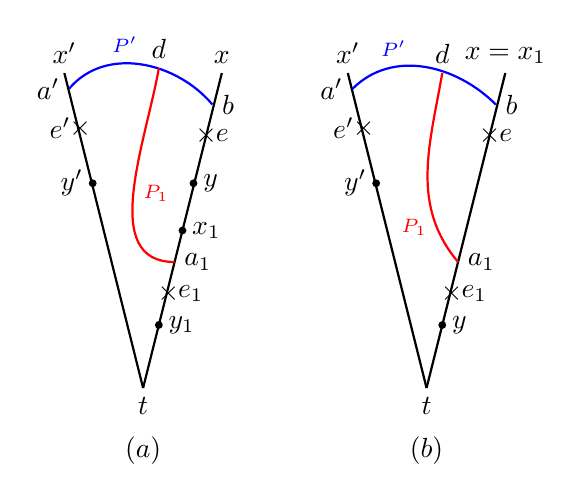
\begin{tikzpicture}[scale=2]
\begin{scope}
\coordinate (s) at (0.5,2);
\coordinate (s1) at (-0.5,2);
%\coordinate (s2) at (1.1,2);
%\coordinate (w) at (0.5,1.4);
\coordinate (t) at (0,0);
\coordinate (ts) at (0.15,0.4);
\coordinate (b) at (0.44,1.8);
\coordinate (y1) at (-0.32,1.3);
\coordinate (y) at (0.32,1.3);

\coordinate (x2) at (0.25,1);
\coordinate (y2) at (0.1,0.4);

\coordinate (a1) at (-0.47,1.9);
\coordinate (a2) at (0.2,0.8);
\coordinate (v) at (0.4,1.6);
\coordinate (v1) at (-0.4,1.65);
\coordinate (v2) at (0.16,0.6);
\coordinate (c) at (-0.7,0.66);
\coordinate (d) at (0.1,2.03);

\draw[thick](s)--(t);
\draw[thick](s1)--(t);
%\draw[thick](s2)--(w);
%\draw[thick](w)--(t);
\node[above] at (s){$x$};
\node[above] at (s1){$x'$};
%\node[above] at (s2){$s_1$};
\node[below] at (t){$t$};
\node[left] at (a1){$a'$};
\node[right] at (b){$b$};

\node[above] at (d){$d$};
%\node[right] at (w){$w$};


\draw[blue,thick] (a1) to[out=50,in=130]
node[pos=0.4,above]
{\scriptsize  $P'$}  (b);



\draw[red,thick] (a2) to[out=180,in=260]
node[pos=0.5,right]
{\scriptsize  $P_1$}  (d);

\node at (v1){$\times$};
\node[left] at (v1){$e'$};


\node[right] at (a2){$a_1$};

\node at (v){$\times$};
\node[right] at (v){$e$};

\node at (v2){$\times$};
\node[right] at (v2){$e_1$};

%\node at (ts){$\times$};
%\node[right] at (ts){$t_{s}$};

\draw (y1) node[fill,circle,scale=0.3]{};
\node[left] at (y1){$y'$};

\draw (y) node[fill,circle,scale=0.3]{};
\node[right] at (y){$y$};

\draw (x2) node[fill,circle,scale=0.3]{};
\node[right] at (x2){$x_1$};

\draw (y2) node[fill,circle,scale=0.3]{};
\node[right] at (y2){$y_1$};

\node at (0,-0.4){$(a)$};

\end{scope}
\begin{scope}[xshift=1.8cm]
\coordinate (s) at (-0.5,2);
\coordinate (s1) at (0.5,2);

\coordinate (t) at (0,0);
\coordinate (ts) at (0.1,0.4);
\coordinate (b) at (0.44,1.8);

\coordinate (a2) at (0.2,0.8);
\coordinate (d) at (0.1,2);
\coordinate (y1) at (-0.32,1.3);
\coordinate (y) at (0.1,0.4);
\coordinate (a1) at (-0.47,1.9);
\coordinate (a) at (0.1,0.8);
\coordinate (v) at (0.4,1.6);
\coordinate (v2) at (0.16,0.6);
\coordinate (v1) at (-0.4,1.65);
\coordinate (c) at (-0.7,0.66);

\draw[thick](s)--(t);
\draw[thick](s1)--(t);

\node[above] at (s){$x'$};
\node[above] at (s1){$x=x_1$};
\node[below] at (t){$t$};
\node[left] at (a1){$a'$};

\node[right] at (b){$b$};
\node[right] at (a2){$a_1$};
\node[above] at (d){$d$};

\draw[blue,thick] (a1) to[out=45,in=135]
node[pos=0.3,above]
{\scriptsize  $P'$}  (b);


\draw[red,thick] (a2) to[out=130,in=260]
node[pos=0.2,left]
{\scriptsize  $P_1$}  (d);

\node at (v1){$\times$};
\node[left] at (v1){$e'$};

\node at (v2){$\times$};
\node[right] at (v2){$e_1$};

\node at (v){$\times$};
\node[right] at (v){$e$};



\draw (y1) node[fill,circle,scale=0.3]{};
\node[left] at (y1){$y'$};

\draw (y) node[fill,circle,scale=0.3]{};
\node[right] at (y){$y$};

\node at (0,-0.4){$(b)$};
\end{scope}
\end{tikzpicture}
\caption{Two cases in which $P'$ passes through $e_1$ after intersecting with $P_1$}
\label{fig:badexample}

\end{figure}
